\documentclass[a4paper]{report}
\usepackage[utf8]{inputenc}
\usepackage[portuguese]{babel}
\usepackage{hyperref}
\usepackage{a4wide}
\hypersetup{pdftitle={Dotprod},
pdfauthor={João Teixeira, José Ferreira, Miguel Solino},
colorlinks=true,
urlcolor=blue,
linkcolor=black}
\usepackage{subcaption}
\usepackage[cache=false]{minted}
\usepackage{listings}
\usepackage{booktabs}
\usepackage{multirow}
\usepackage{appendix}
\usepackage{tikz}
\usepackage{authblk}
\usepackage{bashful}
\usepackage{verbatim}
\usepackage{amssymb}
\usepackage{multirow}
\usepackage{mwe}
\usepackage[parfill]{parskip}
\usetikzlibrary{positioning,automata,decorations.markings}
\AfterEndEnvironment{figure}{\noindent\ignorespaces}
\AfterEndEnvironment{table}{\noindent\ignorespaces}

\usepackage{titlesec}

\titleformat{\chapter}[display]
   {\normalfont\large\bfseries}{\chaptertitlename\ \thechapter}{0pt}{\huge}
\titlespacing*{\chapter}{0pt}{0pt}{0pt}

\begin{document}

\title{Laboratórios de Engenharia Informática\\Projeto 93 - Carage}
\author{João Teixeira (A85504) \and José Filipe Ferreira (A83683) \and Miguel Solino (A86435)}
\date{\today}

\begin{center}
    \begin{minipage}{0.75\linewidth}
        \centering
        
\includegraphics[width=0.4\textwidth]{images/eng.jpeg}\par\vspace{1cm}
        \vspace{1.5cm}
        \href{https://www.uminho.pt/PT}
        {\color{black}{\scshape\LARGE Universidade do Minho}} \par
        \vspace{1cm}
        \href{https://www.di.uminho.pt/}
        {\color{black}{\scshape\Large Departamento de Informática}} \par
        \vspace{1.5cm}
        \maketitle
    \end{minipage}
\end{center}

\begin{abstract}
    \begin{center}
        Ao longo deste relatório iremos descrever e documentar o processo
        de criação de uma plataforma digital Web e Mobile em modo PWA com a
        capacidade para gestão, compra e venda de automóveis com um componente
        de \textit{machine learning} para calcular o valor do automóvel no
        momento da venda.
    \end{center}
\end{abstract}

\tableofcontents

\chapter{Introdução}

O mercado automóvel e uma área em crescimento constante: Existem
mais de 290 milhões de carros na União Europeia e no ano de 2019 foram
vendidos mais de 15 milhões de automóveis novos. No entanto, gerir uma
frota automóvel revela-se extremamente difícil. Organizar todas as
despesas de cada carro e interpretar essa informação de forma útil requer o
uso de ferramentas não intuitivas que tradicionalmente estão renegadas ao
reino da contabilidade de uma empresa. Por isso, tanto uma pessoa que tenha
mais do que um carro como uma pequena empresa tem imensas dificuldades em
gerir os custos da sua frota automóvel.

Com a idade media dos automóveis a aumentar todos os anos, o mercado de
carros usados encontra-se definitivamente em florescimento. Infelizmente,
quando finalmente chega a altura de vender os carros para adquirir novas
viaturas, estimar o preço de cada uma requer um conhecimento técnico
e uma investigação cuidada por parte do proprietário que a maioria
simplesmente não tem a disponibilidade para fazer.

A nossa \textit{web app} propõe-se a resolver estes dois problemas numa
plataforma só que junta a compra, venda e gestão de automóveis. Um utilizador
pode adicionar os seus automóveis, associar de forma intuitiva despesas correntes
e receber estatísticas sobre os custos totais de forma sucinta e clara. Quando
o utilizador finalmente quiser vender um dos seus carros, um algoritmo de \textit{machine
learning} estima o valor de mercado para que seja possível vender o carro  na
plataforma de venda integrada ao melhor preço possível, mas mesmo assim competitivo
com o mercado actual. Este mesmo algoritmo e usado para auxiliar os compradores
a saberem se o preço do carro em que estão interessados em comprar esta dentro
da media do mercado.

Ao longo deste relatório iremos descrever as tecnologias utilizadas e a estrutura deste
aplicação revolucionaria colocando um foco no desenvolvimento do \textit{machine learning}
para previsão de preços.

\chapter{Estudo de Mercado}

Fazendo uma pesquisa de eventuais concorrentes descobrimos que existem algumas
plataformas de vendas de carros usados no mercado. Exemplos destas São o StandVirtual,
o \url{auto.sapo.pt} e o Olx. Porem, existem algumas falhas em todas estas plataformas.
O Olx e uma plataforma generalista de venda de qualquer produto e, por isso, não inspira
a confiança necessária para um comprador em busca de um carro usado.
O auto.sapo.pt não apresenta qualquer tipo de previsão de preço tanto para
o vendedor como para o comprador. O StandVirtual e a plataforma que mais se aproxima do
nosso componente de venda de automóveis pois apresenta uma indicação a possíveis compradores
se o preço do carro esta acima da media. No entanto, a data deste relatório, não apresenta
qualquer tipo de sugestão de preço aquando da venda do carro.

No departamento de gestão de uma frota automóvel: as poucas aplicacoes moveis existentes tem
interfaces gráficas desactualizadas e não existem \textit{web apps} no mercado. Desta forma
não existe nenhuma solução para gestão de automóveis que seja transversal a todos os dispositivos.

Por outro lado, não existe qualquer plataforma digital no mercado que funda a vertente de gestão
e a vertente de compra e venda, fazendo com que este projeto apresente uma embalagem única de
funcionalidades.

\chapter{Backend}

\section{Tecnologias Utilizadas}

O backend foi escrito na linguagem de programação \href{http://rust-lang.org}{Rust}, escolhida
pela sua capacidade de garantir correção do código aquando da compilação, sendo menos propicio
a existência de bugs, aliada à boa documentação e existência de frameworks úteis ao projeto.

Para o motor da base de dados, escolhemos uma base de dados relacional \textit{postgres}, visto
que é o mais popular motor de base de dados utilizado atualmente.

\section{Base de dados}

\begin{figure}[H]
    \centering
    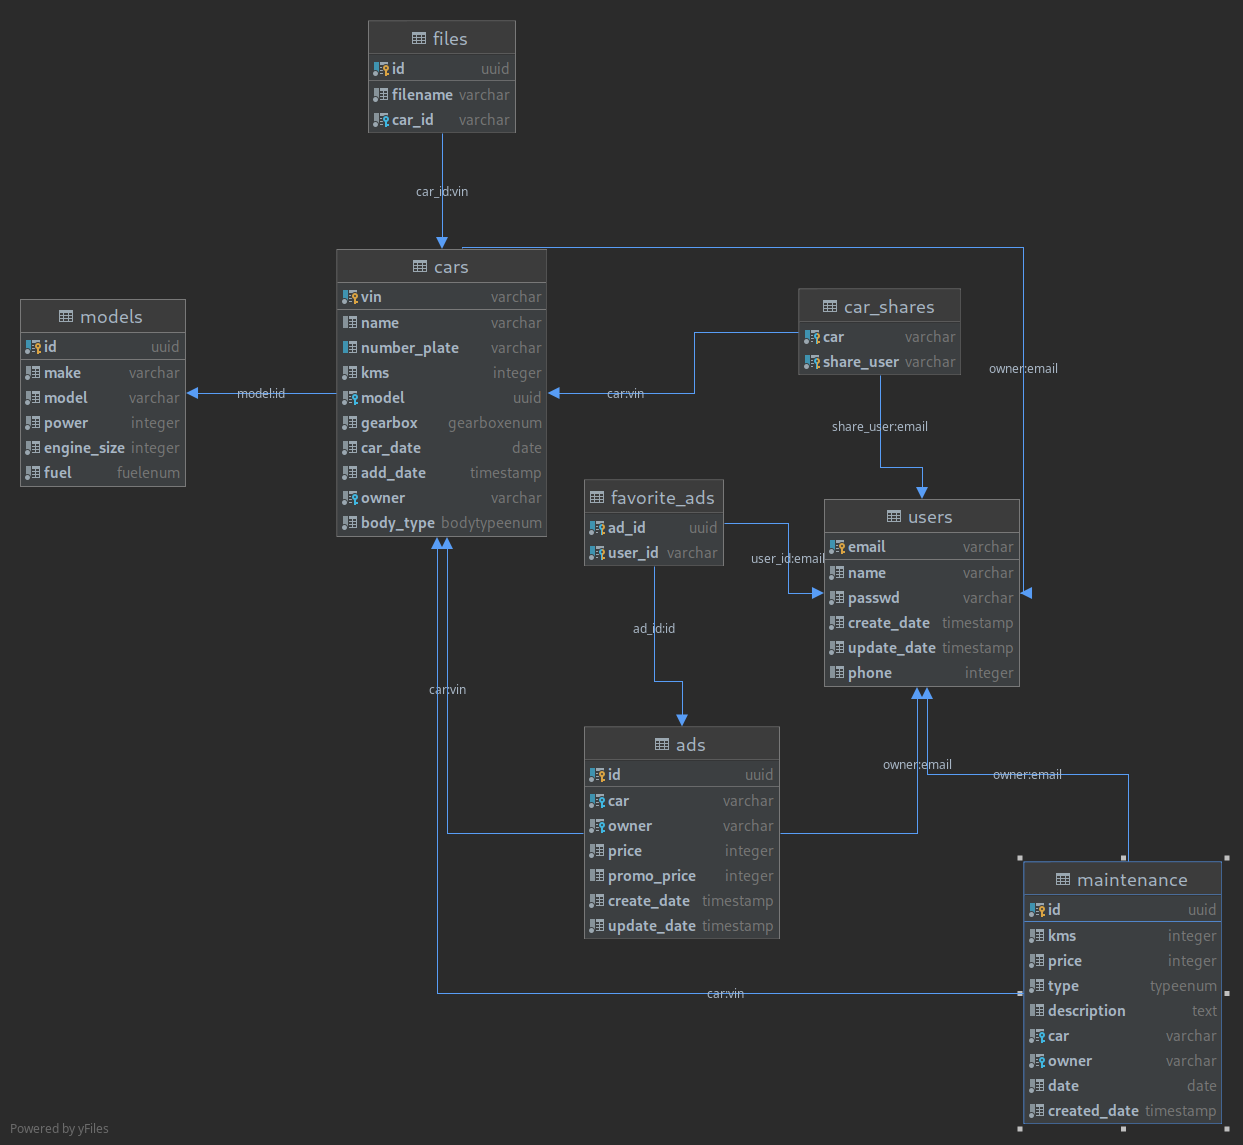
\includegraphics[width=\textwidth]{images/database.png}
    \caption{Modelo da base de dados}
\end{figure}

\subsection{Conexão da Base de Dados}

A conexão do backend à base de dados, é efetuada através da framework de \textit{ORM (Object-Relational Mapping)} 
\href{http://diesel.rs}{diesel}, disponivel para a linguagem de programação \href{http://rust-lang.org}{Rust}.
Esta facilita a manipulação de dados na base de dados, pois apresenta uma abstração das queries SQL para código.

\subsection{Users}

Esta tabela contem a informação de todos os utilizadores registados no sistema. 
É aqui que são armazenadas as informações de contacto, bem como as suas credenciais de acesso.

\subsection{Models}

Esta tabela contem a informação dos modelos de veículos que podem inseridos no sistema.
Visto que é uma informação que iria ser comum a muitos veículos, foi abstraída para esta
tabela. É previamente populada, com base na informação presente no dataset recolhido para a
previsão de preços, neste momento com mais de 4000 modelos distintos, para
proporcionar uma melhor e mais facilitada experiência de inserção de carros por parte do
utilizador final.

\subsection{Cars}

Esta tabela contem a informação especifica dos veículos do utilizador final, que consiste na 
quilometragem, tipo de caixa de velocidade, data da primeira matricula, matricula, tipo de automóvel,
se é um carro, carrinha ou SUV, por exemplo.

\subsection{Maintenances}

Tabela que guarda a informação sobre despesas e manutenções de cada carro, nomeadamente, a
quilometragem na qual foi efetuada, data e tipo de despesa, identificando se foi uma
manutenção regular, de prevenção, mudança de pneus, combustível ou avaria.

\subsection{Ads}

Tabela que guarda a informação de um anuncio de um carro, contendo o identificador
do veiculo ao qual se refere, ao utilizador que criou o anuncio, bem como o seu preço
e data de inserção no sistema.

\section{Autenticação do Utilizador}

Por forma a simplificar a gestão do utilizador que faz os pedidos,
implementamos um sistema de tokens, assente no standard \textit{JSON Web
Token} (\textit{JWT}), que contém informação sobre o utilizador e uma assinatura 
digital que marca a autenticidade do mesmo, não dando assim acessos indevidos às 
páginas privadas do utilizador. Este token é gerado aquando da validação das credenciais
no login, e deve estar presente no header do pedido \textit{HTTP} para valiadção.

\section{Comunicação com o Backend}

Para a comunicação do exterior com o backend da aplicação, este expõe uma \textit{REST API},
que apresenta endpoints para a manipulação dos dados guardados no sistema por parte do utilizador,
de forma a manter a segurança e integridade da informação existente. Esta API funciona assente na
framework \href{http://rocket.rs}{rocket}.

\chapter{Previsão de Preços}

Ao longo deste capitulo iremos descrever como desenvolvemos um algoritmo de
\textit{machine learning} com a capacidade de ter em conta o maior numero de factores
possíveis para calcular o valor de mercado de um carro usado.

\section {Obtenção de Dados}

Para treinar este algoritmo precisamos de obter um \textit{dataset} considerável de
carros usados. Para tal usamos a maior plataforma de venda de carros usados em Portugal:
o Standvirtual.

Para a obtenção dos dados decidimos utilizar uma linguagem de scripting, neste caso Javascript,
de forma a que este processo fosse direto e pouco demorado. 
Inicialmente foi necessária uma análise de como o StandVirtual esta organizado 
relativamente a componentes HTML. Munidos desta informação e fazendo uso da biblioteca 
\textit{Cheerio} de Javascript conseguimos manusear o HTML completo de forma a retirar
apenas as informações relevantes sobre os dados dos carros.
Este script vai página a página, obtém a lista de carros nessa página e extrai,
carro a carro, as informações respectivas. Devido ao rate limiting incutido pela api do
standvirtual apenas conseguimos obter dois carros por segundo levando a que o processo todo
demore aproximadamente oito horas.

\section{Análise dos Dados}

Começando por uma análise geral dos dados, as informações que extraímos de cada carro
foram:
\begin{itemize}
    \item \textbf{brand} - Marca;
    \item \textbf{model} - Modelo;
    \item \textbf{version} - Sub-modelo;
    \item \textbf{fuel} - Tipo de combustível;
    \item \textbf{month} - Mês de produção;
    \item \textbf{year} - Ano de produção;
    \item \textbf{km} - Quilómetros totais percorridos;
    \item \textbf{displacement} - Cilindrada do motor;
    \item \textbf{power} - Potência em cavalos;
    \item \textbf{gearbox} - Tipo de caixa;
    \item \textbf{doors} - Número de portas;
    \item \textbf{seats} - Número de lugares;
    \item \textbf{origin} - Nacional ou Importado;
    \item \textbf{price} - Preço de venda;
\end{itemize}

Como resultado final obtivemos 46713 carros com um total de 14 colunas e tamanho de
ficheiro 5 MiB, existindo alguns valores em falta.

\begin{figure}[H]
    \centering
    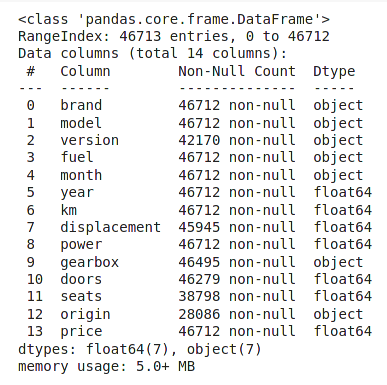
\includegraphics[width=0.5\textwidth]{images/data_understanding.png}
    \caption{Informações gerais do dataset obtido}
\end{figure}

Com o objetivo de ter os melhores resultados possíveis, passamos também por um processo
de análise mais profundo. Ou seja, avaliamos quais São os factores que mais afectam o preço
com base nas correlacoes representadas através de heatmaps.

\begin{figure}[H]
    \centering
    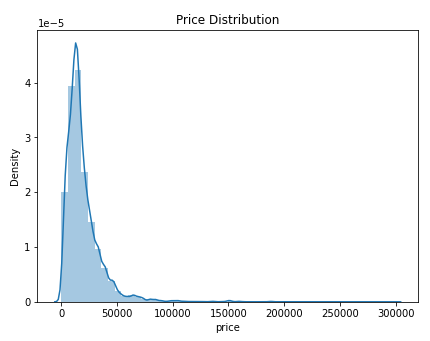
\includegraphics[width=0.6\textwidth]{images/price_density.png}
    \caption{Densidade dos preços}
\end{figure}

\begin{figure}[H]
    \centering
    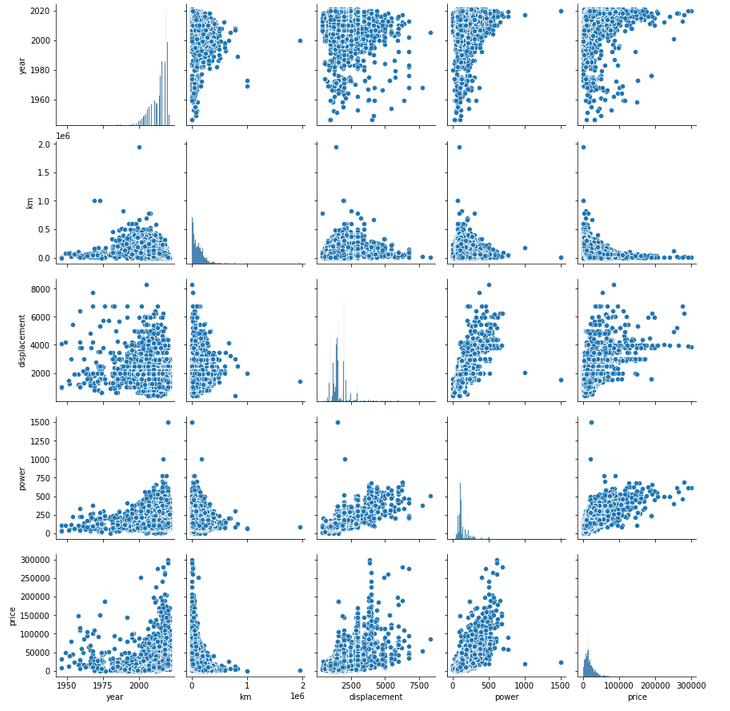
\includegraphics[width=\textwidth]{images/correlation.png}
    \caption{Correlação dos dados com mais impacto}
\end{figure}

\begin{figure}[H]
    \centering
    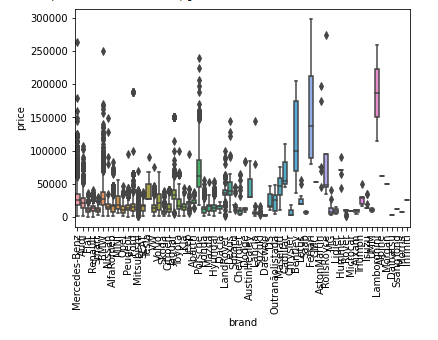
\includegraphics[width=0.6\textwidth]{images/price_brands.png}
    \caption{Distribuição dos preços pelas marcas}
\end{figure}

\begin{figure}[H]
    \centering
    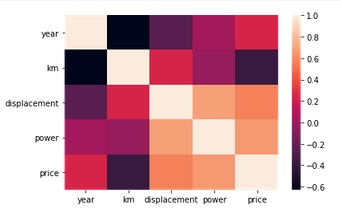
\includegraphics[width=0.6\textwidth]{images/heatmap.png}
    \caption{Correlação em Heatmap dos dados com mais impacto}
\end{figure}

Visualizando estes dois últimos gráficos chegamos à conclusão que os atributos com maior 
relevância para o nosso modelo são: brand, fuel, year, km, displacement, power e gearbox.
Infelizmente, nem todos os gráficos analisados por nós são legíveis
e por isso não achamos relevante colocar. Isto deve-se a alguns valores em falta e por
maior parte dos campos serem nominais com valores únicos quase na sua totalidade.

\section{Preparação dos Dados}

Com uma análise feita e sabendo quais os dados que são obrigatórios usarmos, passamos à 
preparação dos mesmos para mais à frente aplicarmos o modelo.
Como referido anteriormente, para uma melhora dos resultados foram separadas as colunas com
maior impacto no preço, resultando no seguinte processo aplicado nos dados:
\begin{itemize}
    \item \textbf{Remoção de atributos} - Remoção das colunas dos dados com menos impacto no
    preço sobrando as referidas na secção anterior;
    \item \textbf{Conversão dos dados} - Tendo em conta que vários dos dados são nominais e 
    estes algoritmos não suportam valores não-numéricos, foi feita uma conversão dos dados 
    originando colunas do tipo "boolean";
    \item \textbf{Remoção de valores em falta} - Como se trata de previsão de preços e o
    nosso objetivo é obter os melhores resultados possíveis, não podemos inventar valores 
    que alterem a exactidão das previsões. Assim sendo removemos todas as linhas que 
    continham valores em falta.
\end{itemize}

Abaixo estão presentes pedaços de código executados no Google Colab referentes 
a cada uma das etapas do processo.

\begin{figure}[H]
    \centering
    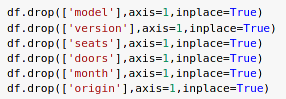
\includegraphics[width=0.5\textwidth]{images/drop_values.png}
    \caption{Remoção das colunas com pouca relevância}
\end{figure}

\begin{figure}[H]
    \centering
    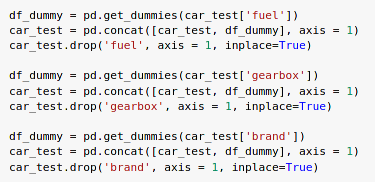
\includegraphics[width=0.5\textwidth]{images/remove_dummies.png}
    \caption{Conversão dos dados nominais para númericos}
\end{figure}

\begin{figure}[H]
    \centering
    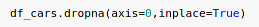
\includegraphics[width=0.5\textwidth]{images/remove_missing.png}
    \caption{Remoção das linhas com dados em falta}
\end{figure}

\section{Aplicação dos Modelos e Resultados}

Tendo em mãos os dados preparados, passamos à fase de treino e teste do dataset para cada
algoritmo. Visto que tradicionalmente este tipo de situacoes São tratadas por algoritmos de
regressão foi por ai que começamos a nossa pesquisa do melhor modelo para prever de preços dos
automóveis.

Inicialmente experimentamos tres algoritmos distintos: Linear Regression, Lasso Regressione
Ridge Regression. Curiosamente estes 3 apresentam resultados muito semelhantes e bastante
abaixo das expectativas. Com uma pesquisa um pouco mais profunda descobrimos um outro tipo
de modelo denominado de XGBoost (Regressor), que para surpresa nossa, foi o que nos ofereceu
de longe os melhores resultados, sendo eles muito superiores aos três anteriores.

\begin{figure}[H]
    \centering
    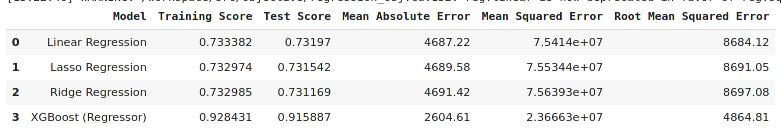
\includegraphics[width=\textwidth]{images/resultados.png}
    \caption{Comparação entre pontuações e erros dos algoritmos usados}
\end{figure}

Tendo em conta estes resultados, decidimos utilizar como algoritmo final o XGBoost, obtendo 
previsão de preços bastante próximos dos reais.

\begin{figure}[H]
    \centering
    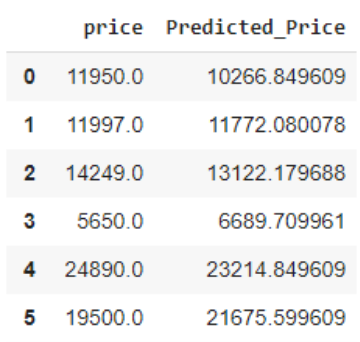
\includegraphics[width=0.4\textwidth]{images/resultados_prices.png}
    \caption{Cinco carros com o preço real e previsto resultante da aplicação do algoritmo}
\end{figure}

\chapter{Frontend}

Relativamente à componente do frontend, esta foi desenvolvida utilizando a framework
\href{http://nextjs.org}{Next.js} e
foram implementadas maior parte das funcionalidades propostas. 
É possível o utilizador criar uma conta na página inicial como também efetuar o login. 

Na dashboard consegue-se visualizar um resumo geral de todos os dados da sua conta, como número de
carros, anúncios, despesas, etc. 

Depois na página de carros é possível criar um carro como aceder a um dos criados ou partilhados. Na
própria página de um carro é possível adicionar manutenções, colocar à venda, partilhar o carro e pedir
uma previsão ou uma estimativa de quanto é que o carro vale atualmente.

Na página de mercado é possível ver todos os anúncios existentes na plataforma e também a possibilidade
de os filtrar por certos atributos. 

Existe também a página de favoritos onde irão aparecer os 
anúncios favoritos e a página de perfil onde é possível editar o nome, password ou número de telemóvel.

É importante referir que a estimativa de preços é usada em duas páginas: a página do próprio carro como
foi referido anteriormente e na página de um anúncio.
Na página do carro esta previsão é dada num intervalo que o carro poderá valer. Já na página de 
anúncios a previsão de preços é utilizada de uma forma diferente, quando o carro está mais barato, mais
caro ou dentro do preço previsto é indicado por baixo do preço dado pelo vendedor essa previsão.

Abaixo estão presentes maior parte das páginas existentes na nossa aplicação.

\section{Página Inicial}

\begin{figure}[H]
    \centering
    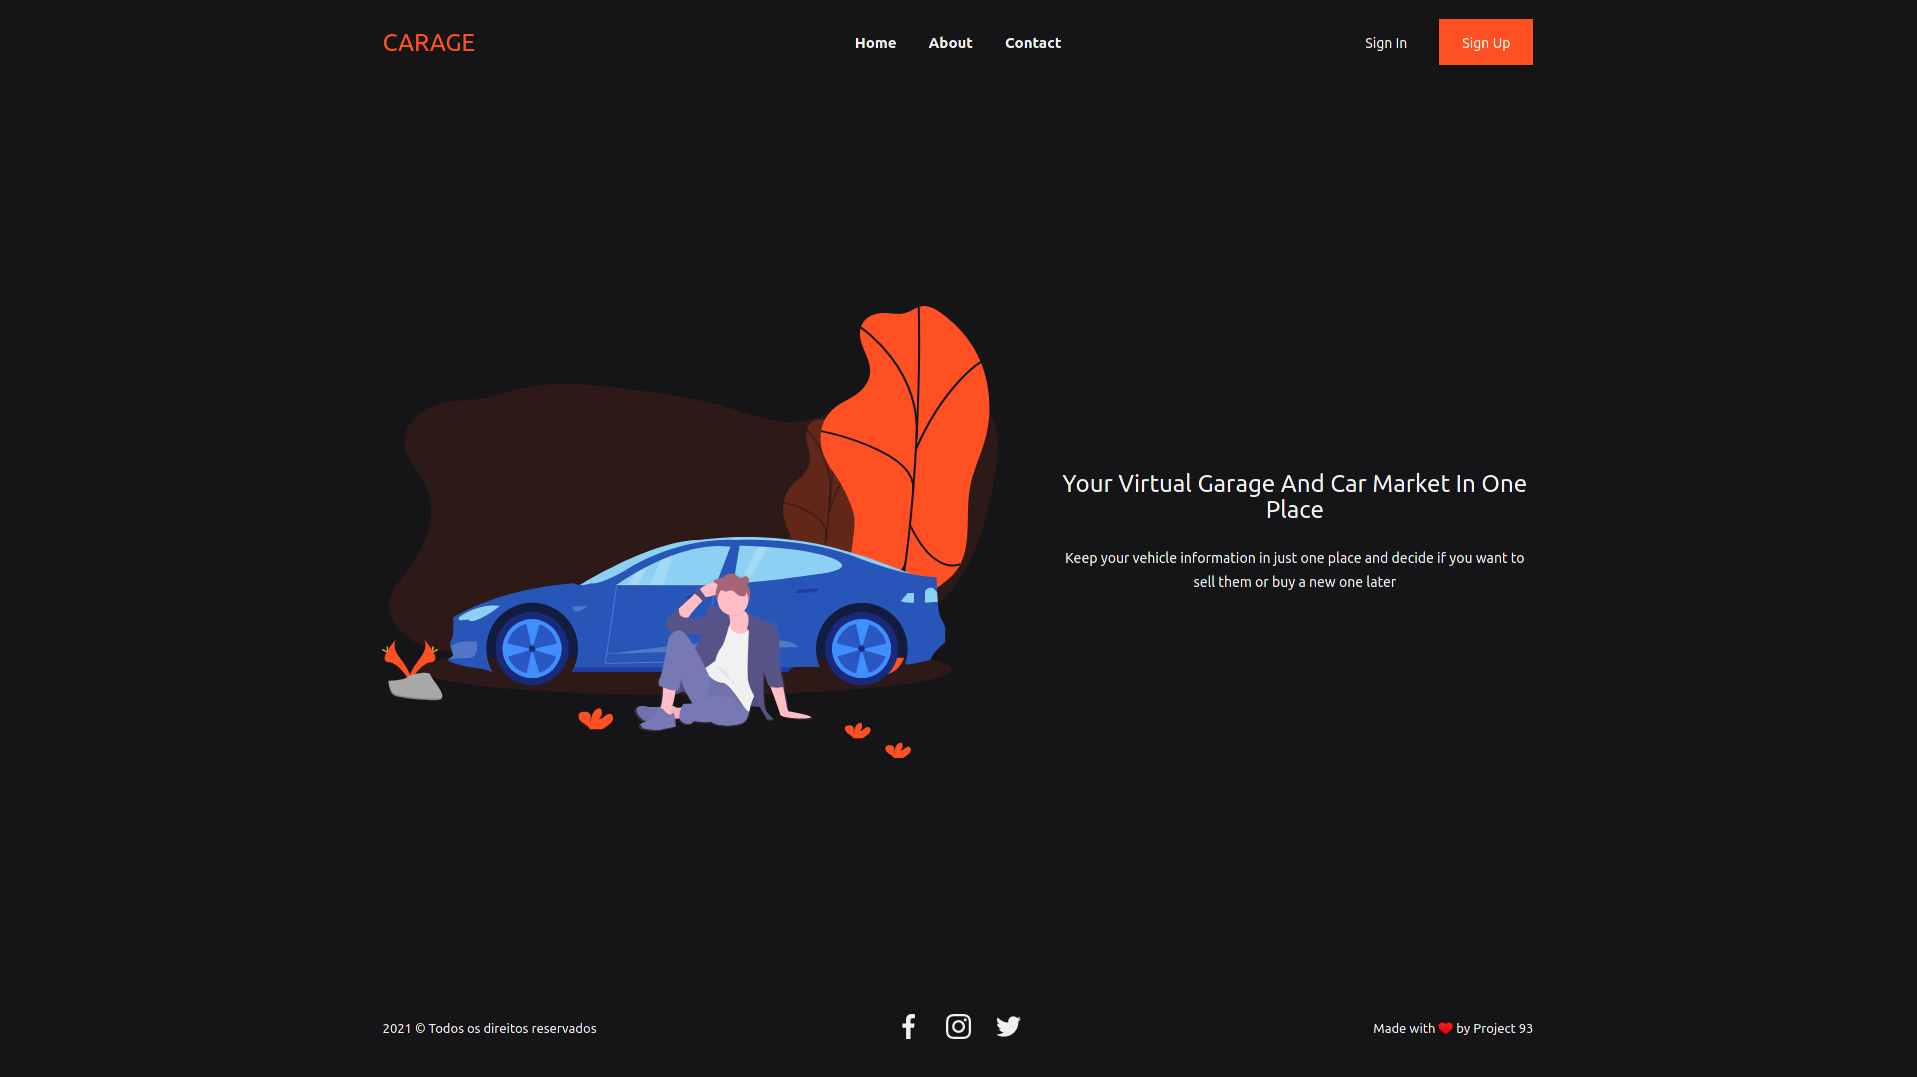
\includegraphics[width=0.9\textwidth]{images/homepage.png}
    \caption{Página inicial desktop}
\end{figure}

\begin{figure}[H]
\centering
\begin{minipage}{.5\textwidth}
  \centering
    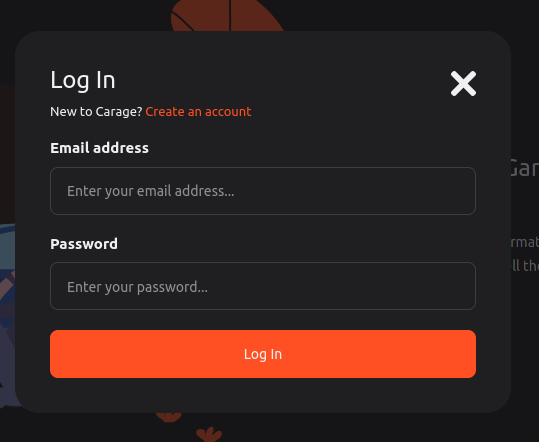
\includegraphics[width=0.7\textwidth]{images/homepage_signin.png}
    \captionof{figure}{Form de login}
\end{minipage}%
\begin{minipage}{.5\textwidth}
  \centering
    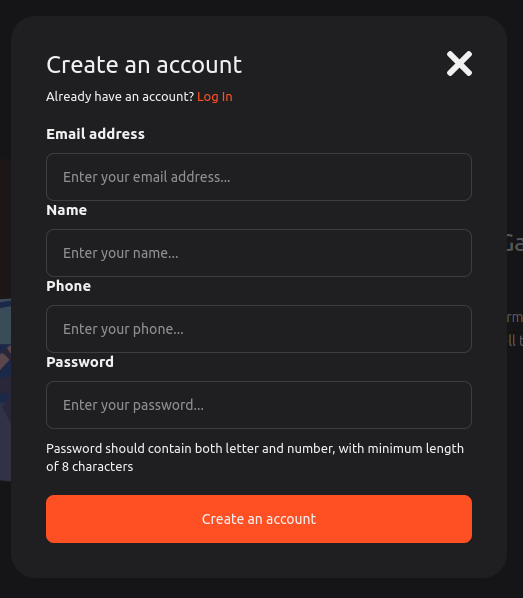
\includegraphics[width=0.7\textwidth]{images/homepage_signup.png}
    \captionof{figure}{Form de registo}
    \label{img:Frame40}
\end{minipage}%
\end{figure}

\begin{figure}[H]
\centering
\begin{minipage}{.5\textwidth}
  \centering
    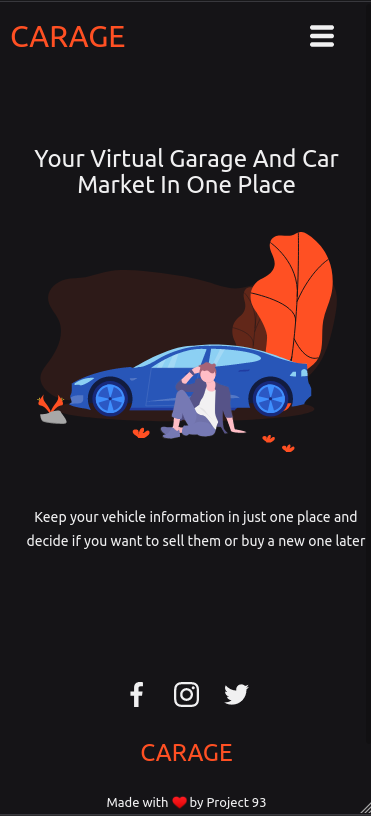
\includegraphics[width=0.7\textwidth]{images/homepage_mobile.png}
    \captionof{figure}{Página inicial mobile}
\end{minipage}%
\begin{minipage}{.5\textwidth}
  \centering
    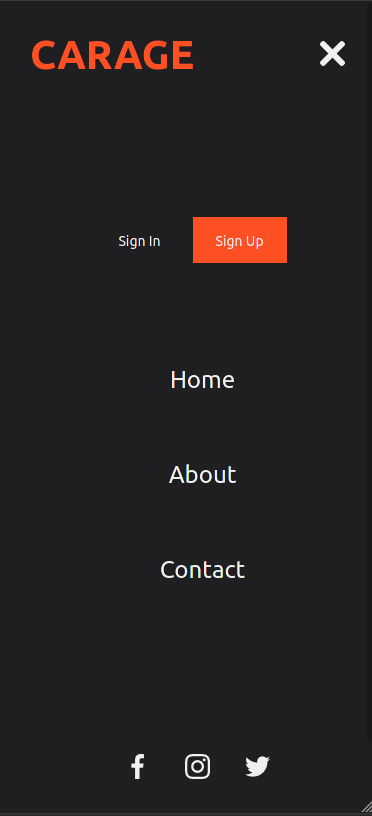
\includegraphics[width=0.7\textwidth]{images/homepage_mobile_menu.png}
    \captionof{figure}{Menu da página inicial mobile}
    \label{img:Frame40}
\end{minipage}%
\end{figure}

\section{Dashboard}

\begin{figure}[H]
    \centering
    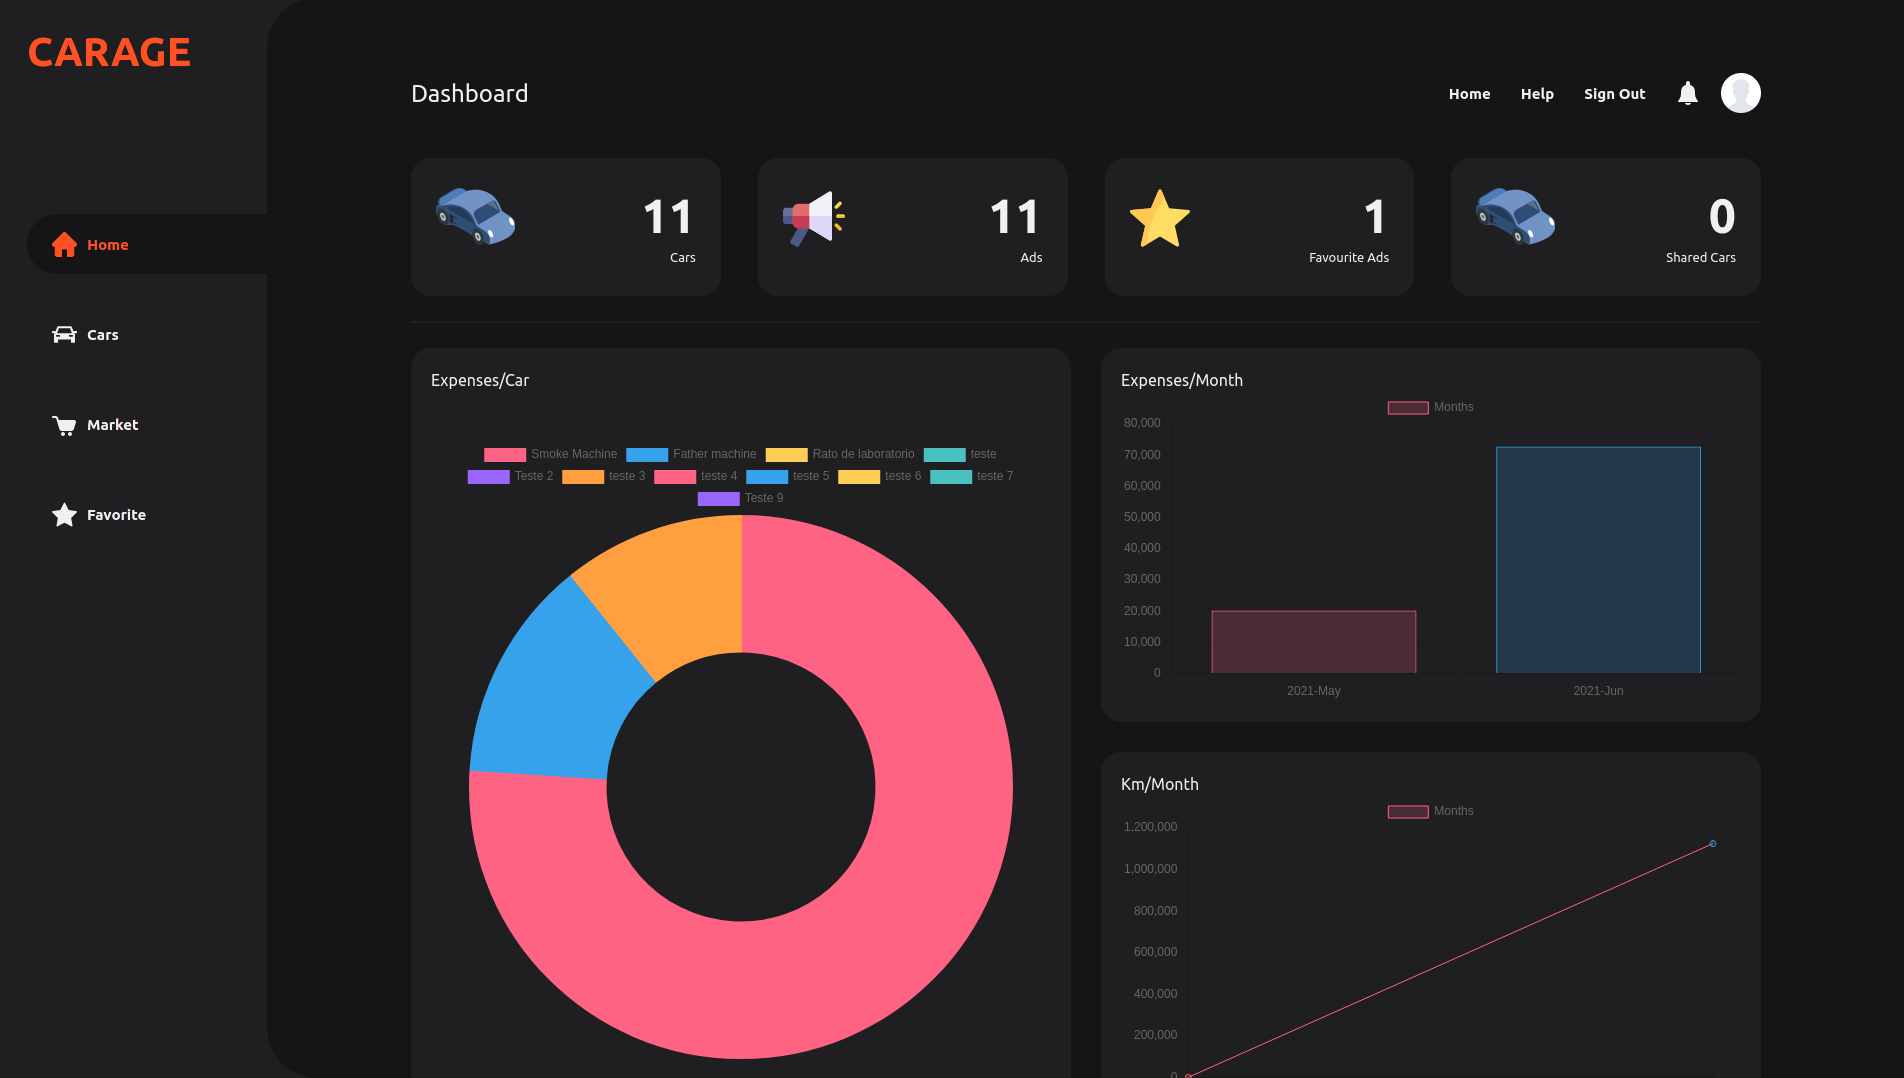
\includegraphics[width=0.9\textwidth]{images/dashboard.png}
    \caption{Dashboard Desktop}
\end{figure}

\begin{figure}[H]
\centering
\begin{minipage}{.5\textwidth}
  \centering
    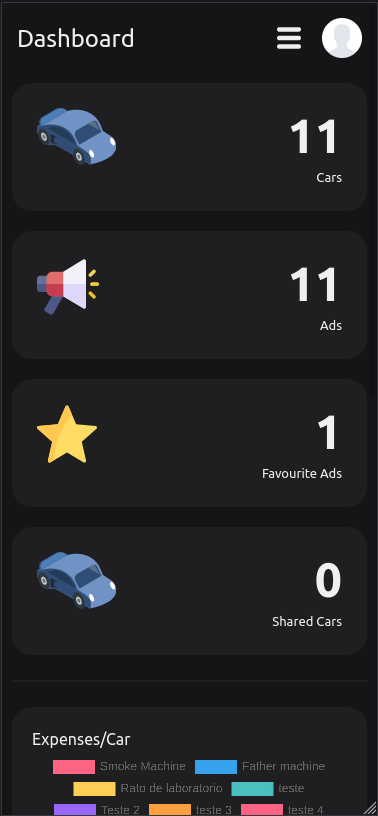
\includegraphics[width=0.7\textwidth]{images/dashboard_mobile.png}
    \captionof{figure}{Dashboard Mobile}
\end{minipage}%
\begin{minipage}{.5\textwidth}
  \centering
    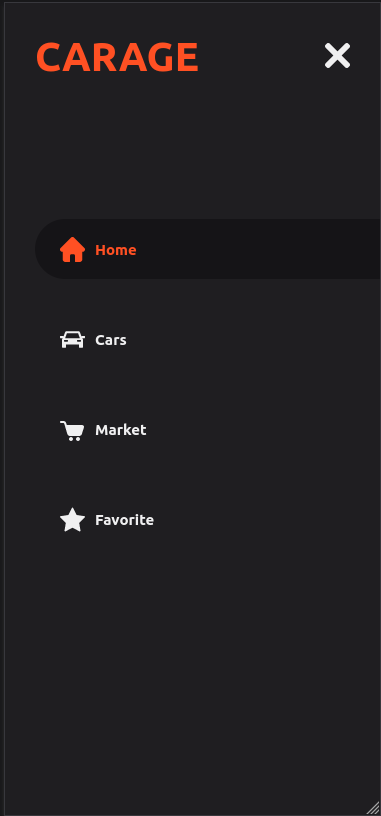
\includegraphics[width=0.7\textwidth]{images/dashboard_mobile_navbar.png}
    \captionof{figure}{Navbar da Dashboard Mobile}
    \label{img:Frame40}
\end{minipage}%
\end{figure}

\pagebreak

\section{Carros}

\begin{figure}[H]
    \centering
    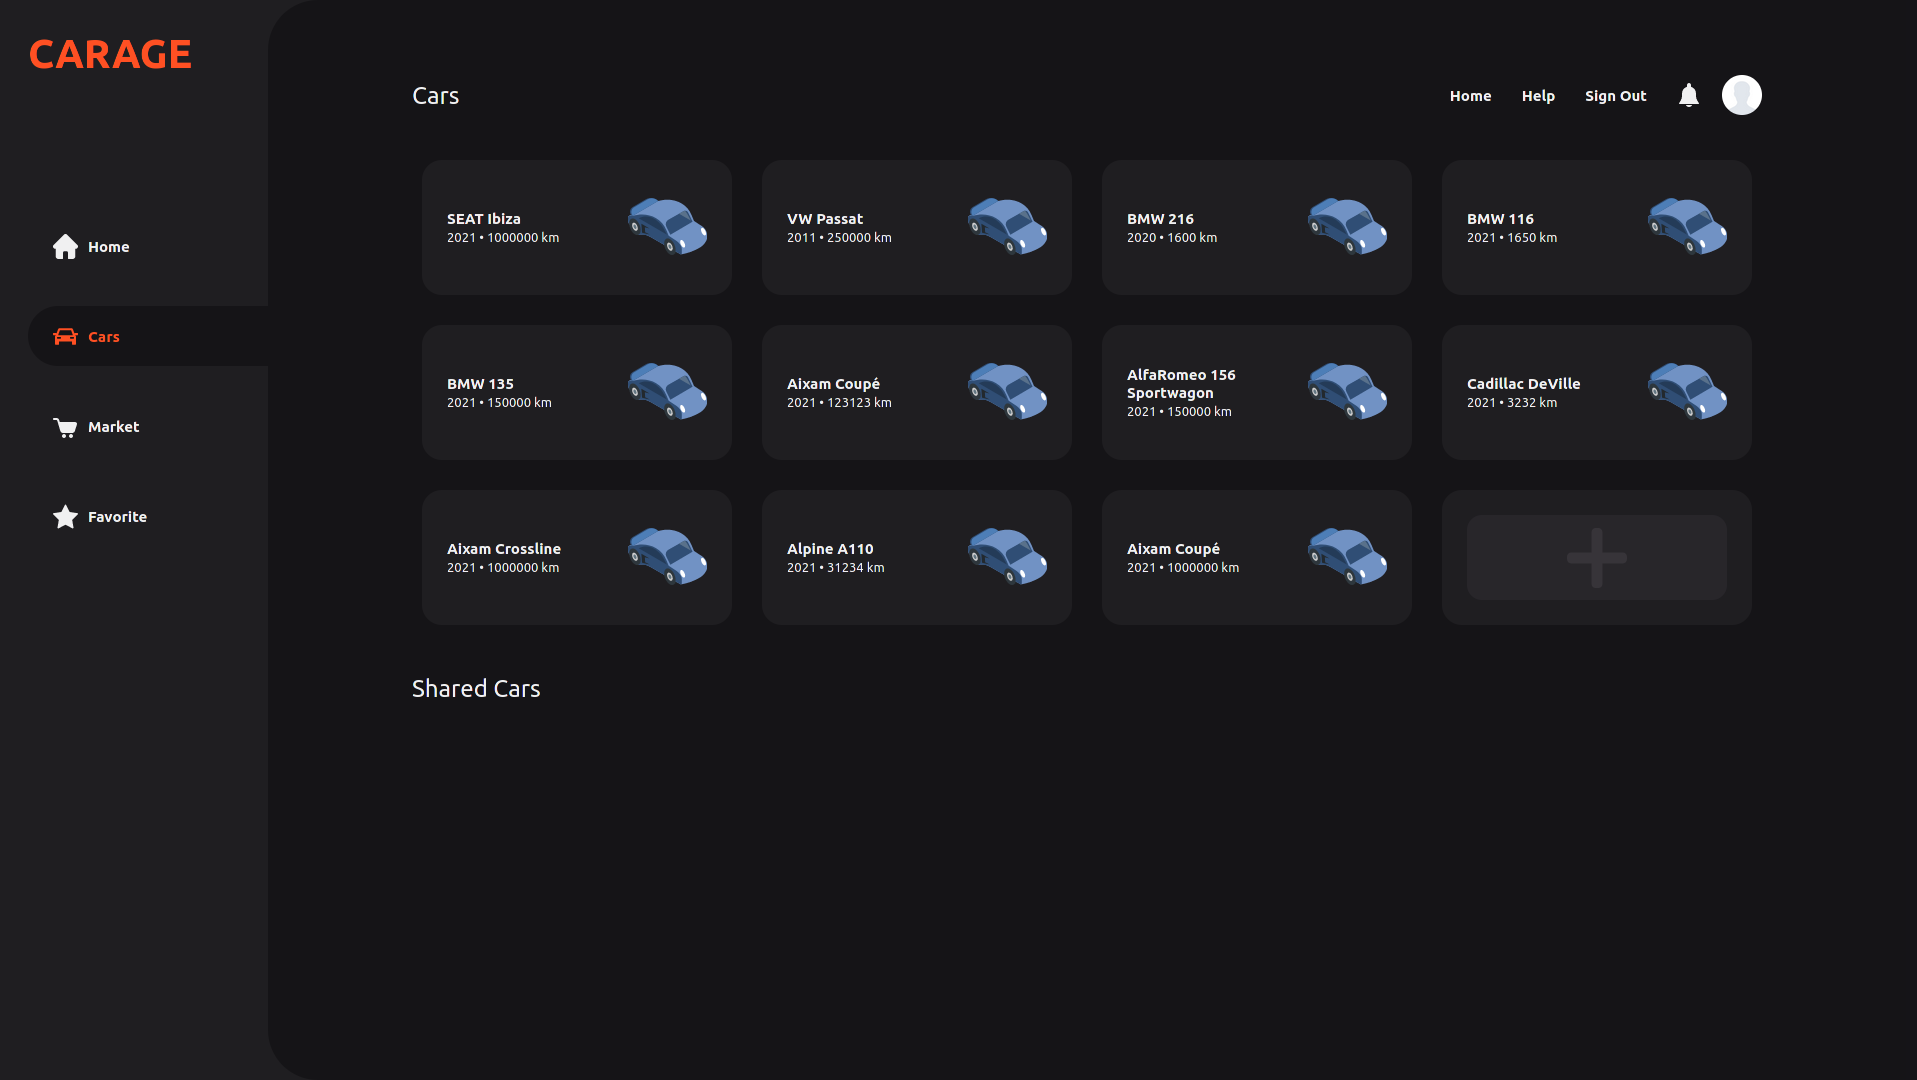
\includegraphics[width=0.9\textwidth]{images/cars.png}
    \caption{Página dos Carros Desktop}
\end{figure}

\begin{figure}[H]
    \centering
    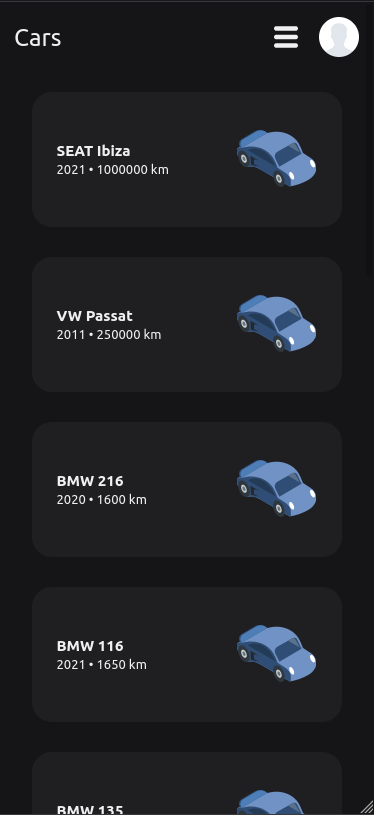
\includegraphics[width=0.35\textwidth]{images/cars_mobile.png}
    \caption{Página dos Carros Mobile}
\end{figure}

\section{Carro}

\begin{figure}[H]
    \centering
    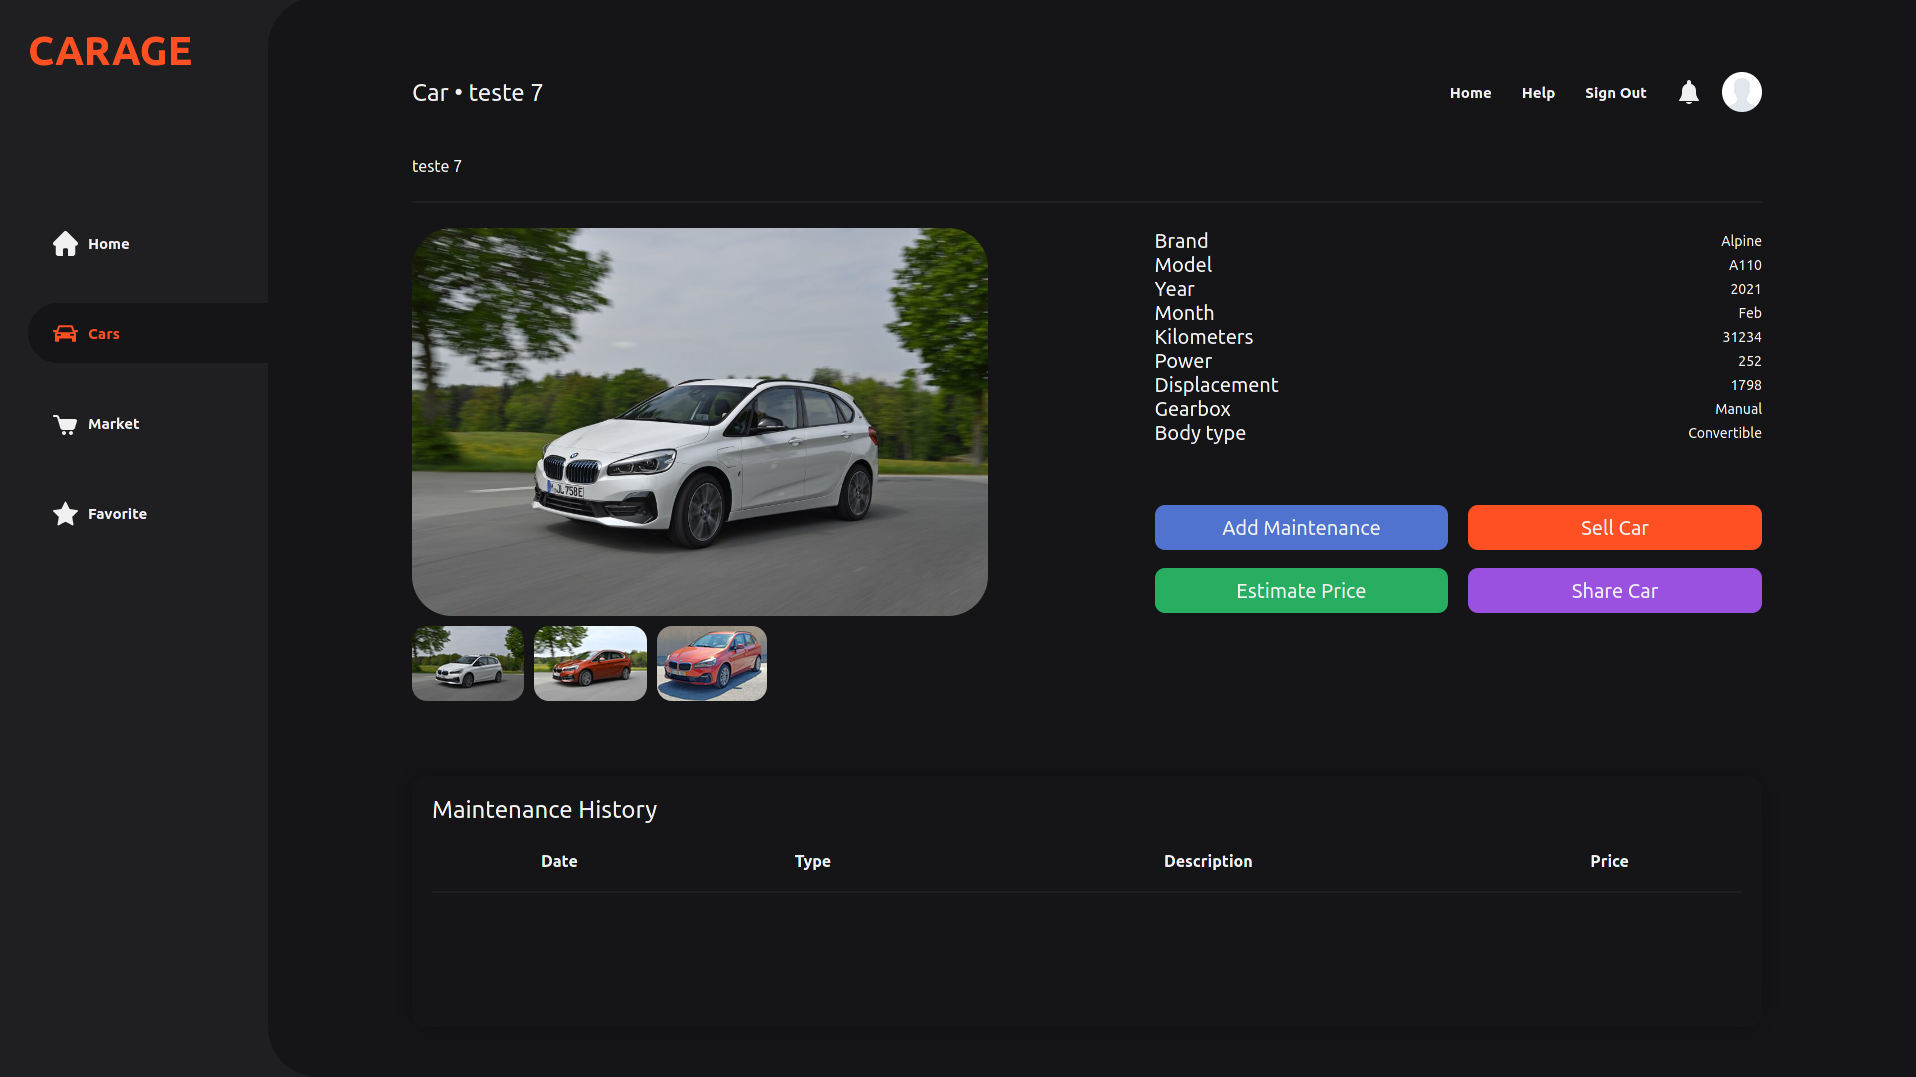
\includegraphics[width=0.9\textwidth]{images/car.png}
    \caption{Página de um Carro Desktop}
\end{figure}

\begin{figure}[H]
    \centering
    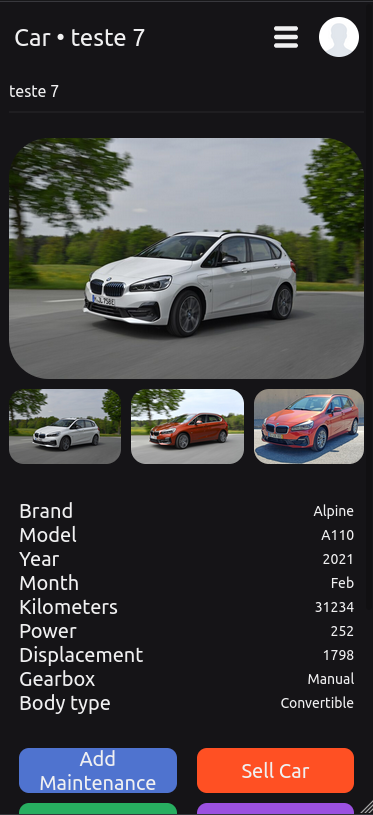
\includegraphics[width=0.35\textwidth]{images/car_mobile.png}
    \caption{Página de um Carro Mobile}
\end{figure}

\section{Mercado}

\begin{figure}[H]
    \centering
    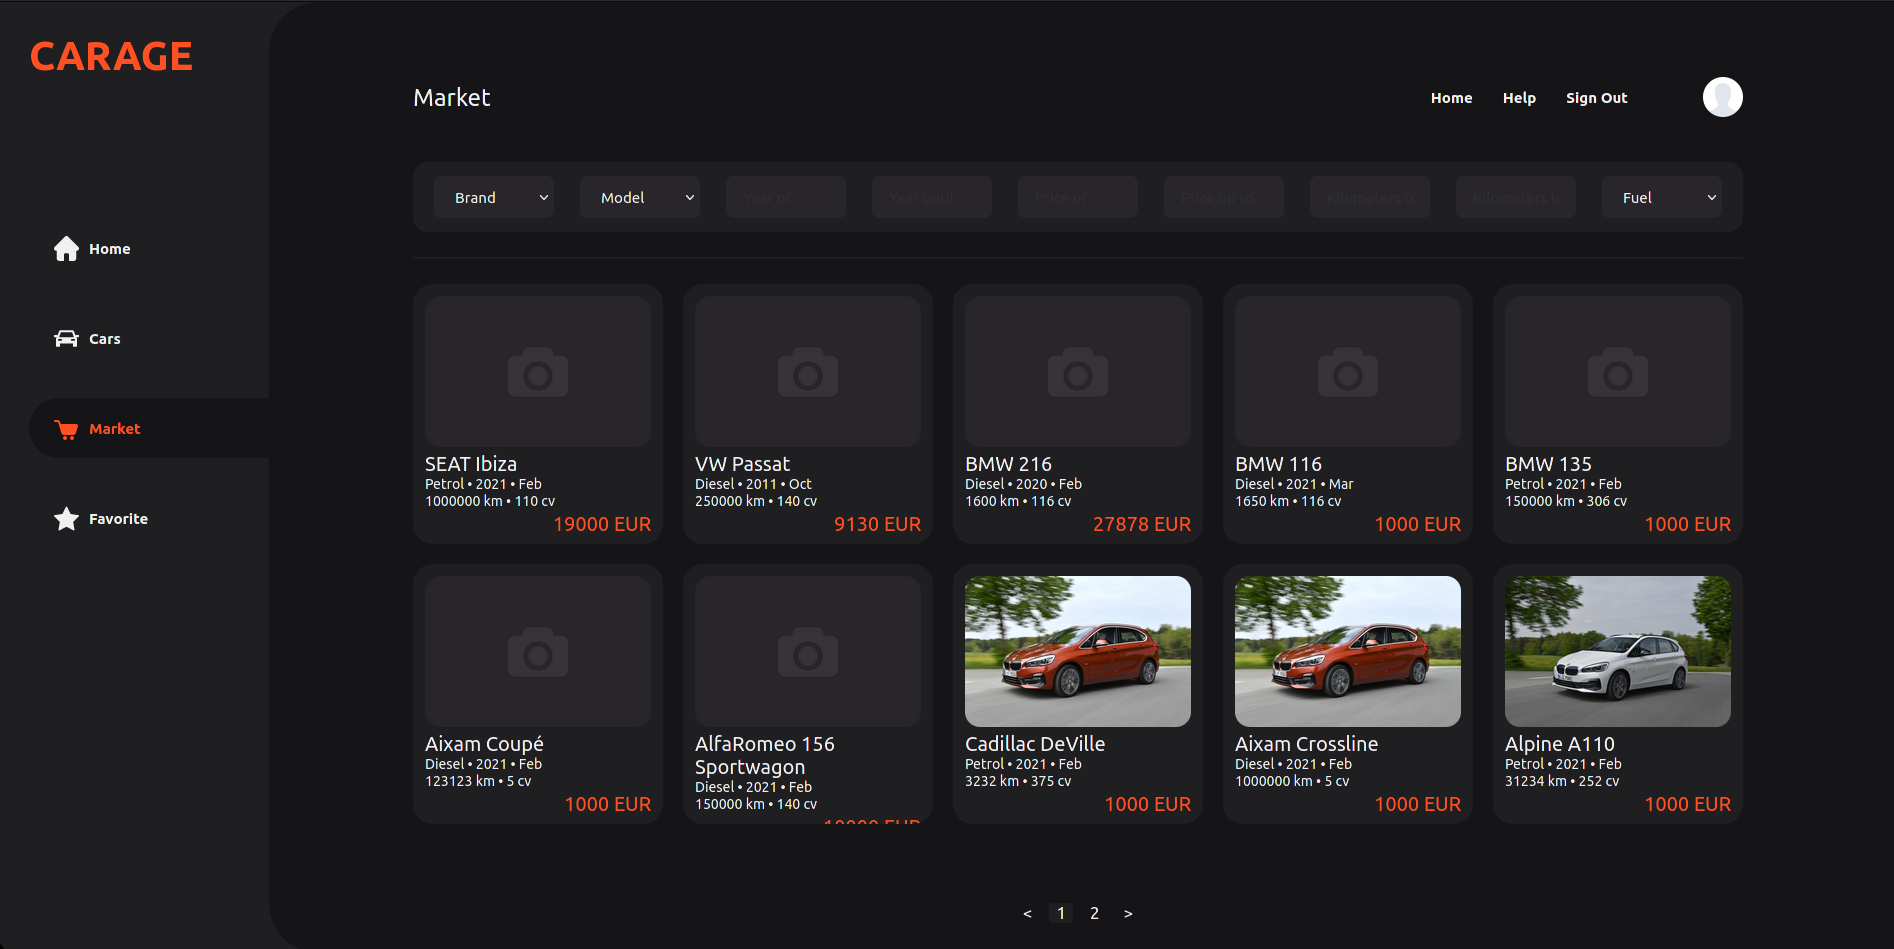
\includegraphics[width=0.9\textwidth]{images/market.png}
    \caption{Página do Mercado Desktop}
\end{figure}

\begin{figure}[H]
    \centering
    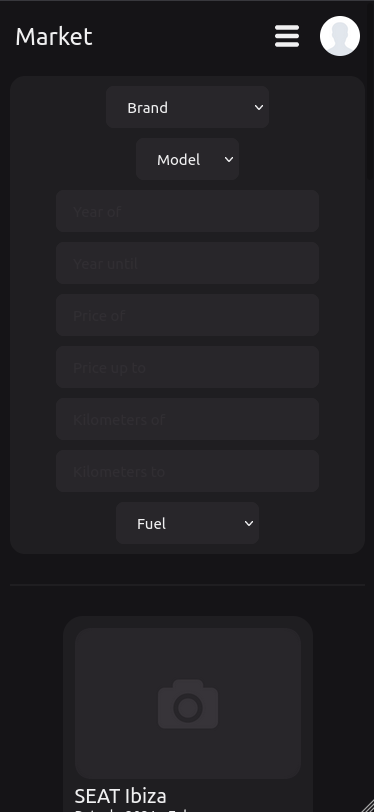
\includegraphics[width=0.35\textwidth]{images/market_mobile.png}
    \caption{Página do Mercado Mobile}
\end{figure}


\section{Anúncio}

\begin{figure}[H]
    \centering
    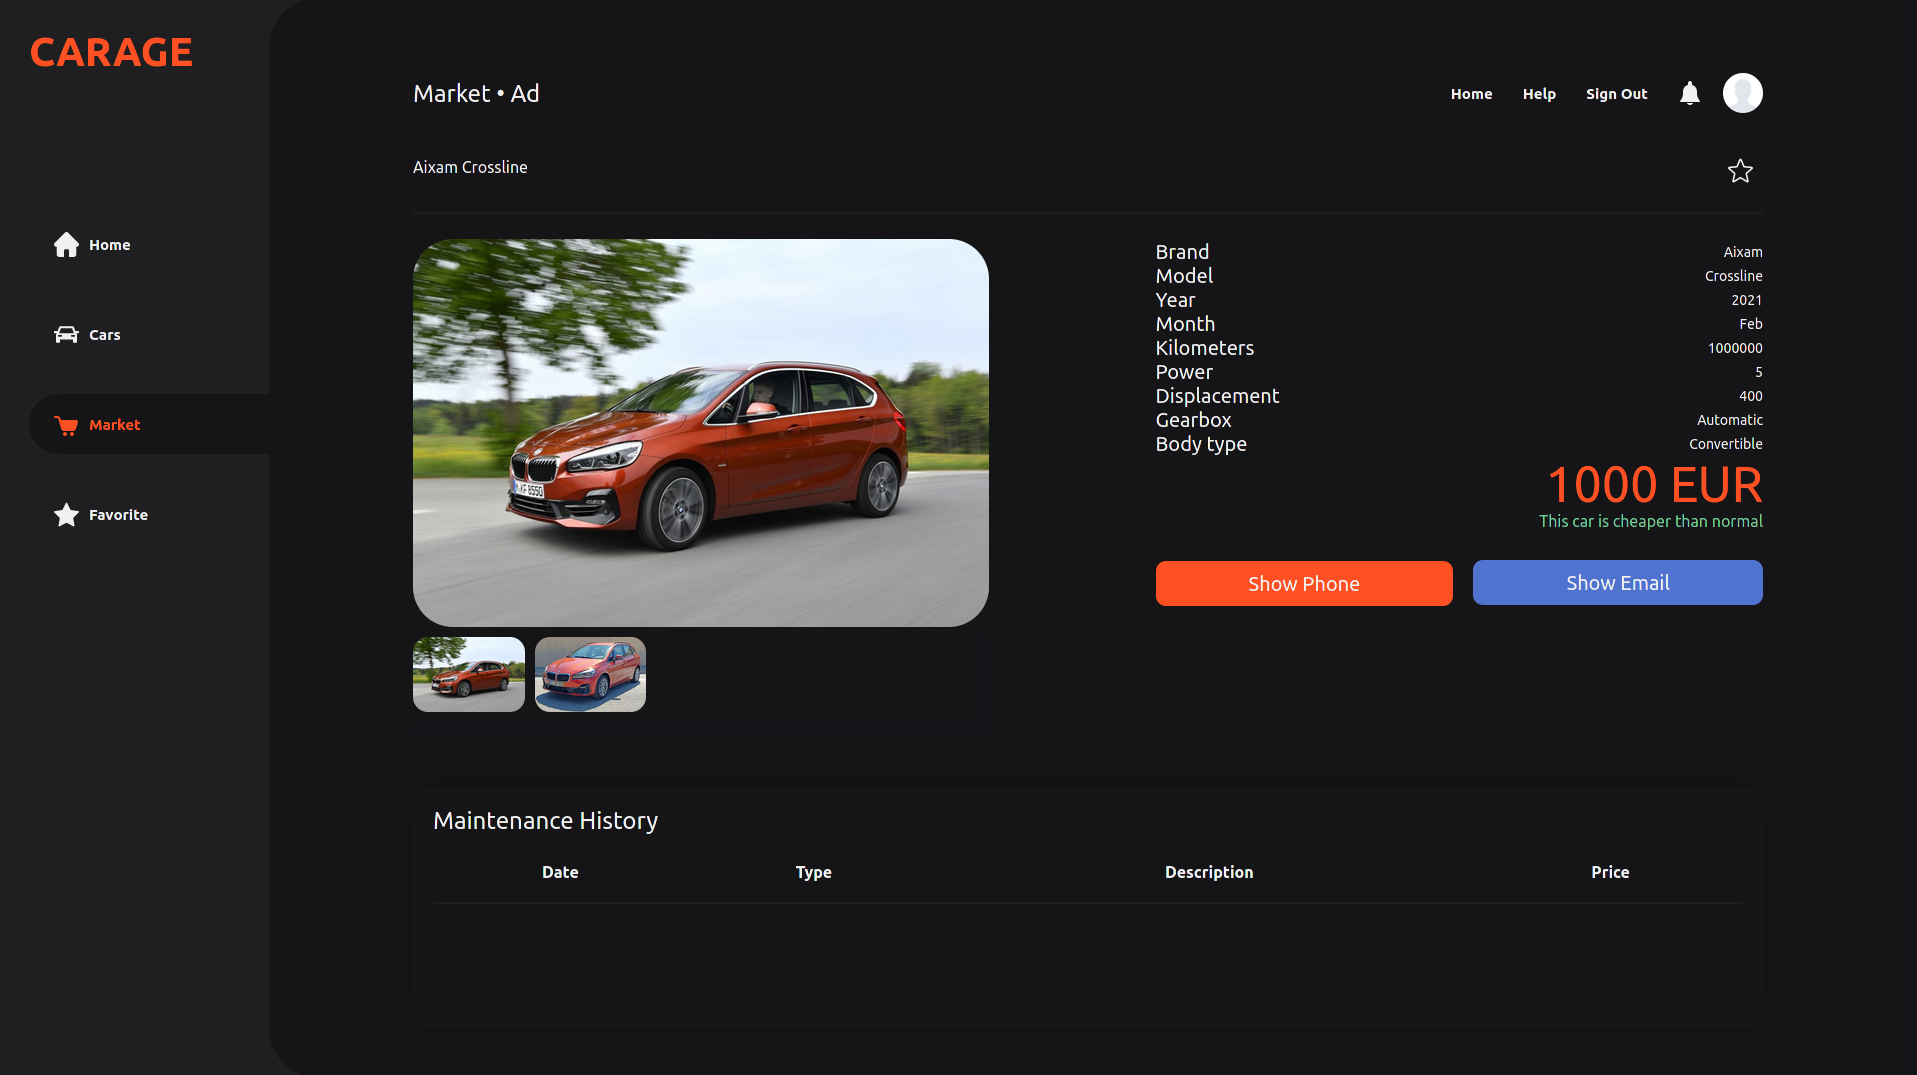
\includegraphics[width=0.9\textwidth]{images/ad.png}
    \caption{Página de um Anúncio Desktop}
\end{figure}

\begin{figure}[H]
    \centering
    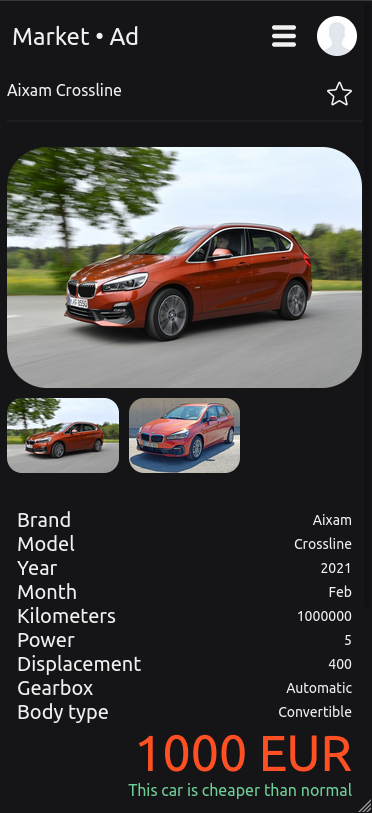
\includegraphics[width=0.35\textwidth]{images/ad_mobile.png}
    \caption{Página de um Anúncio Mobile}
\end{figure}

\chapter{Conclusão e Trabalho Futuro}

Conseguimos cumprir todos os requisitos a que nos propusemos inicialmente
conseguindo realizar com sucesso uma plataforma de gestão compra e venda
de automóveis intuitiva e simples de usar acessível a qualquer pessoa.

Como trabalho futuro gostaríamos de permitir a introdução de um carro
apenas com base na sua matricula e associar fotos ou ficheiros de facturas
aos consumos do carro. Para tal seria necessário expandir as funcionalidades
do armazenamento de ficheiros criado de forma a ser mais genérico e flexível.
Também gostaríamos de apresentar gráficos na pagina de cada carro
semelhantes aos da dashboard. Se este projecto fosse de facto ser utilizado por um
numero elevado de utilizadores também seria necessário fazer um deployment na
cloud, criar uma página de contactos e ajuda funcional e ter um guia de utilizacao
da plataforma quando se entra pela primeira vez.

\end{document}